\documentclass{article}

\usepackage{makecell, graphicx}
\graphicspath{ {./images/} }

\title{Ch. 15 CW \#2 Solutions}
\author{Principles of Microeconomics}
\date{\today}

\begin{document}

\maketitle

\section*{15.2. The Competitive Firm's Supply Curve}

\begin{enumerate}

\item A firm will shut down temporarily if $P < AVC$. If $P < AVC$, then the revenue from producing the typical unit is less than the  variable cost of producing the typical unit. That means the firm is losing more money producing than it would by shutting down. In the short run, fixed costs are unrecoverable whether or not the firm shuts down, so they don't factor into the firm's shut down decision.
	
\item In the summer, lobster is locally available and cheaper. For the rest of the year, the shacks have to source lobster from around the world which is more expensive. Sourcing the lobster from around the world increases the shacks' variable costs. They shut down when their average variable costs are higher than the price that they can receive for their lobster. That's optimal because they save more money (their variable cost) than they give up (their revenue). 

\item A firm will exit a market if $P < ATC$. If $P < ATC$, then the firm's profits are negative. If profits are negative, then the firm will exit the market in the long run.

\item

	\begin{enumerate}
	
	\item $MC$
	
	\item $AVC$
	
	\item $AVC$; $ATC$
	
	\item $ATC$
	
	\end{enumerate}
	
\newpage
	
\item \phantom{x}

	\begin{center}
	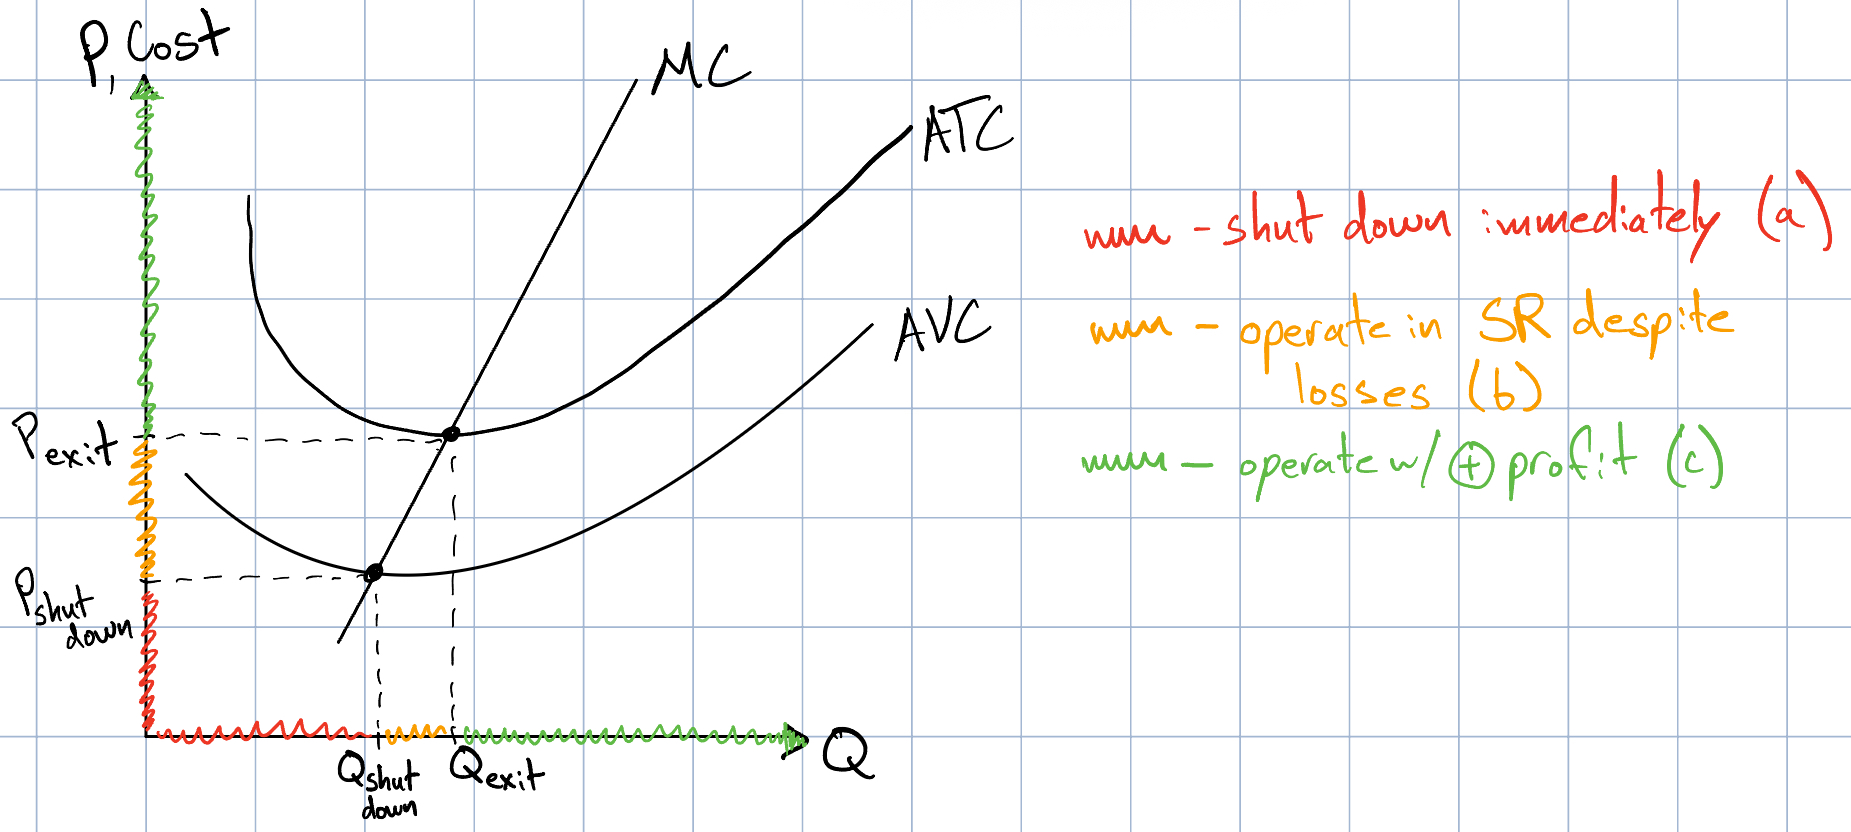
\includegraphics[width = \textwidth]{q5}
	\end{center}
	
\end{enumerate}

\end{document}